\chapter{Проектирование рентгенооптических трактов для Сибирского Кольцевого Источника Фонтов}

\section{Введение}
В данной главе мы рассмотрим схемы рентгенооптических трактов (здесь и далее, - бимлайнов), от источников высокого энергетических фотонов --- вставных устройств до деталей оптических компотен на билайне: фильтров, монохроматоров, рентгеновских зеркал и линз. В этой главе, будут обсуждаться станции первой очереди: 1-1 --- <<Микрофокус>>, 1-2 --- <<Структурная диагностика>>, 1-4 --- <<XAFS-спектроскопия и магнитный дихроизм>>.  
\begin{table}[h!]
	\centering
	\begin{tabular}{c|c|c|c}
		\hline\hline
		%\toprule
		\rule{0pt}{3ex}   $\sigma_x, [m]$ & $\sigma_{x'}, [rad]$ & $\sigma_y, [m]$     & $\sigma_{y'}, [rad]$ \\ \hline
		\rule{0pt}{3ex}   $33.0 \times 10^{-6}$  & $2.65 \times 10^{-6}$  &  $8.6 \times 10^{-7}$ & $5.0 \times 10^{-7}$   \\
		\hline	\hline
		\rule{0pt}{3ex}   $\Delta E / E$ & $\beta_x,[m]$ & $\beta_y,[m]$   & $I,[mA]$\\ \hline
		\rule{0pt}{3ex}	 $8.6 \times 10^{-4}$ & $12.49$ & $1.99$ & $400$ \\ \hline\hline
		%\toprule
	\end{tabular}
	\vspace{4pt} 
	\caption{Параметры накопительного кольца и электронного пучка в ондуляторном пустом промежутке}
	\label{table:ebeam}
\end{table}
На всех указанных станциях будут использоваться сверхпроводящие ондуляторы разработки и производства ИЯФ СО РАН, см., например,  \cite{bragin2018short}, \cite{gluskin2019superconducting}.

\section{Станция 1-1 --- <<Микрофокус>>}
Станция имеет вставное устройство с параметрами указанными в таб.~\ref{table:und1-1}
\begin{table}[h!]
	\centering
	\begin{tabular}{c|c|c|c|c}
		\hline\hline
		\rule{0pt}{3ex}$\mathnormal{B(K), [T]}$   & $\mathnormal{L, [m]}$ & $\mathnormal{d, [mm]}$ & фаз.ошиб.                & Рабочие Гармоники 1-1       \\ \hline
		\rule{0pt}{3ex}$1.36(2.29)$  & $2.3$    & $18$      & $\leq 3^{\circ}$& $11, 13, 17, 23$\\
		\hline\hline
	\end{tabular}
	\vspace{4pt} 
	\caption{Параметры ондулятора для станции 1-1}
	\label{table:und1-1}
\end{table}
при параметрах электронного пучка указанных в таблице~\ref{table:ebeam}: 

\begin{figure}[h!]
	\centering
	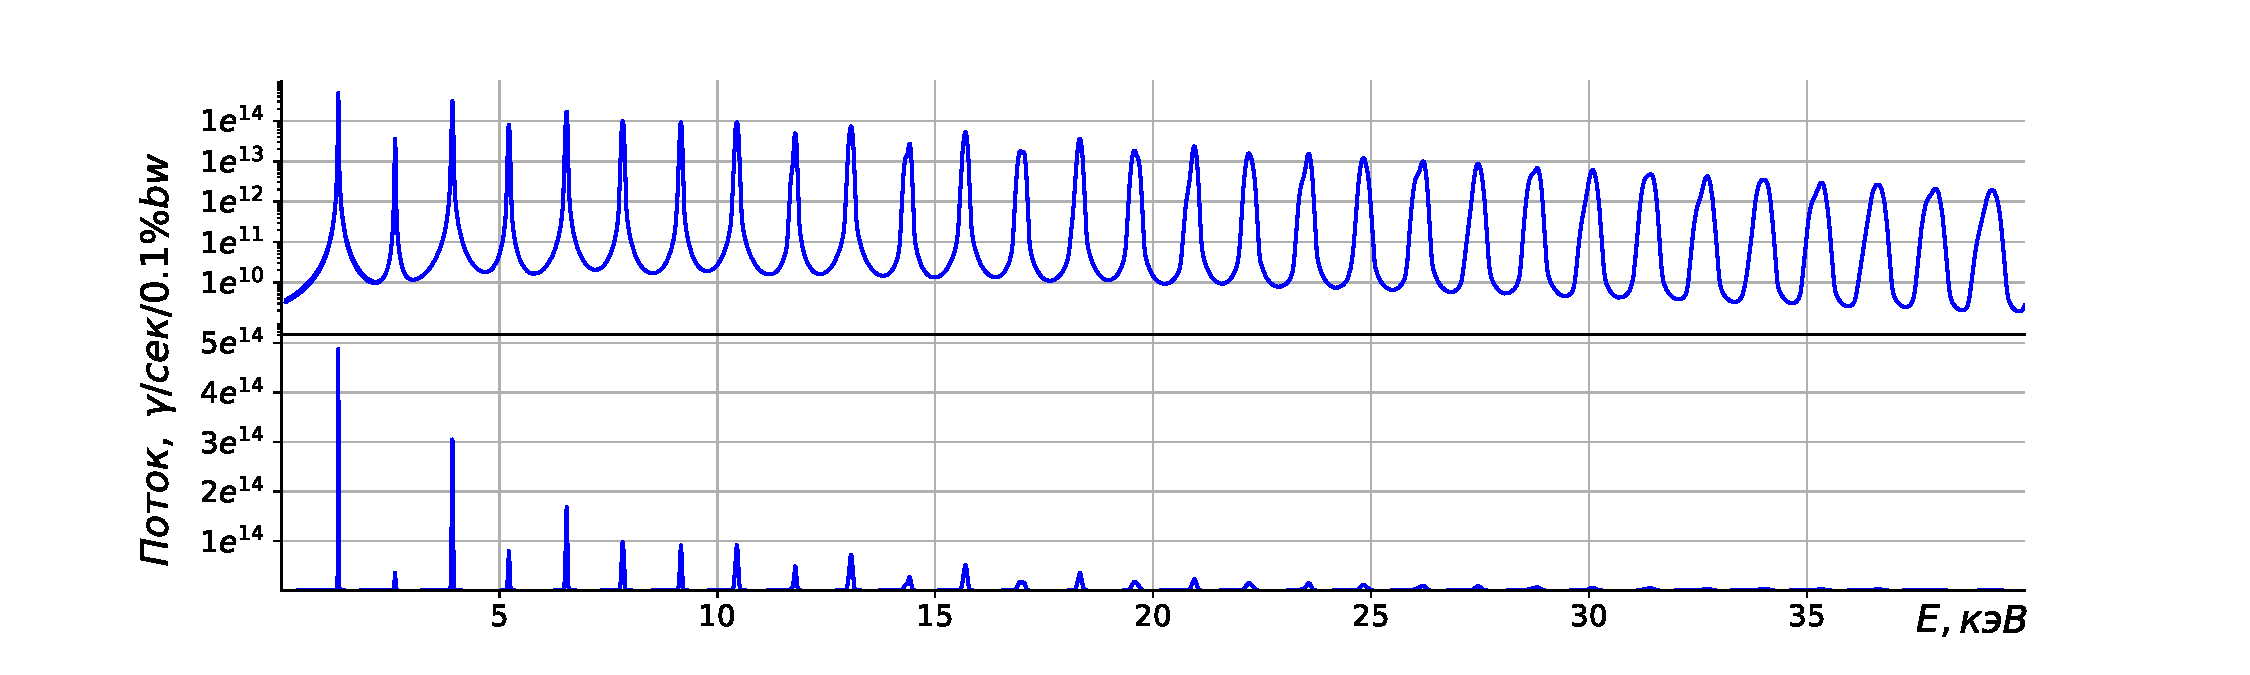
\includegraphics[width=\textwidth]{pic/log_spec_1-1.pdf}
	\caption{Спектр с ондулятора с $K = 2,29$ через апертуру $0,4 \; \textup{мм}$ в логарифмическом масштабе (сверху) и в линейном (снизу) посчитанный в SPECTRA}
	\label{fig:section_und_SRW}
\end{figure}

\subsection{Оптика станции 1-1}

\begin{figure}[h]
	\centering  
	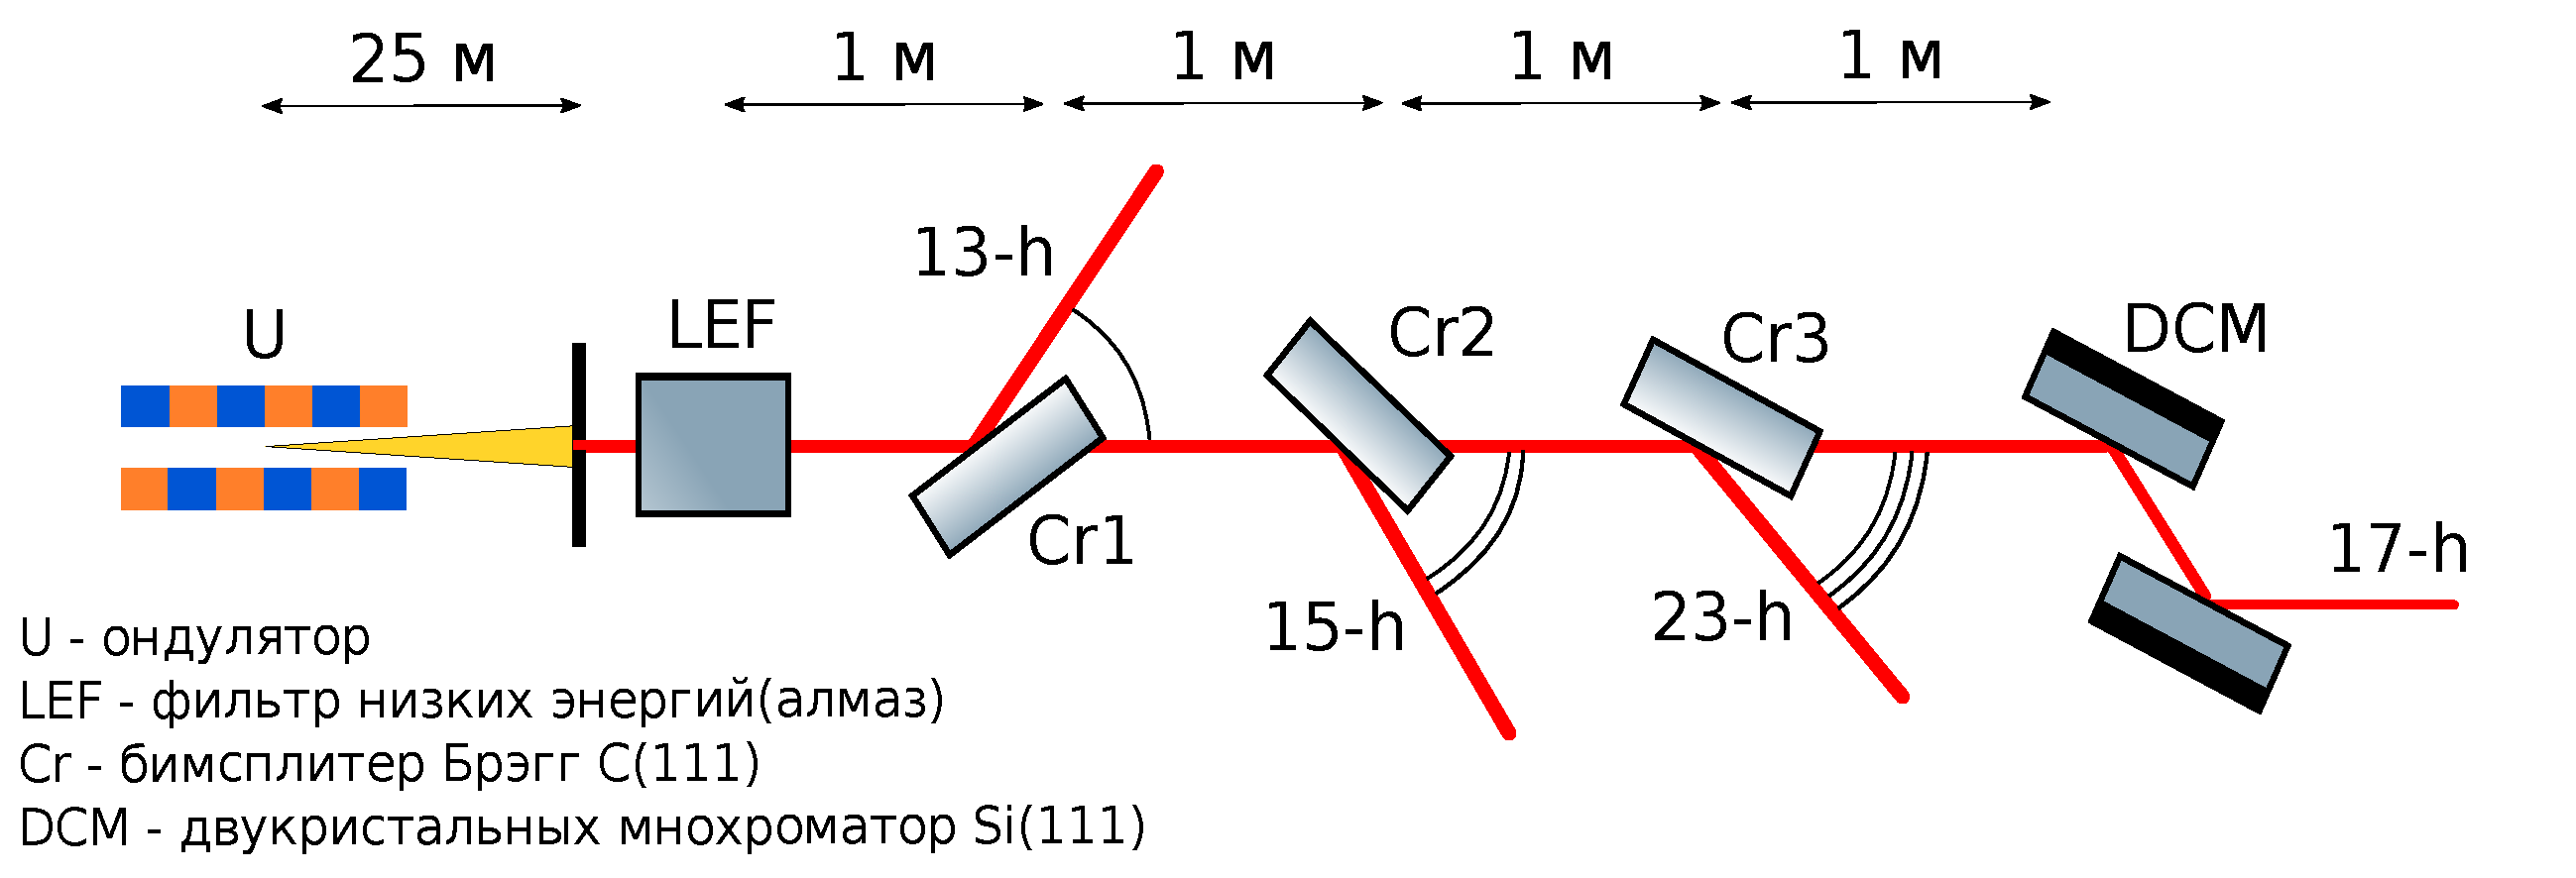
\includegraphics[width=\textwidth]{pic/OptScheme_1-1.pdf}
	\caption{Оптическая схема станции 1-1}
	\label{fig:OptScheme_1-1}  
\end{figure}


\section{Станция 1-2 --- <<Структурная диагностика>>}

\subsection{Вставное устройство}
\begin{table}[h!]
	\centering
	\begin{tabular}{c|c|c|c|c}
		\hline\hline
		\rule{0pt}{3ex}$\mathnormal{B(K), [T]}$   & $\mathnormal{L, [m]}$ & $\mathnormal{d, [mm]}$ & фаз.ошиб.                & Рабочие Гармоники 1-2       \\ \hline
		\rule{0pt}{3ex}$1.06(1.54)$    			  & $2$                   & $15.6$      & $ \leq 3^{\circ}$& $5, 7, 9, 13$\\
		\hline\hline
	\end{tabular}
	\vspace{4pt} 
	\caption{Параметры ондулятора для станции 1-2}
	\label{table:und1-1}
\end{table}

\begin{figure}[h!]
	\centering
	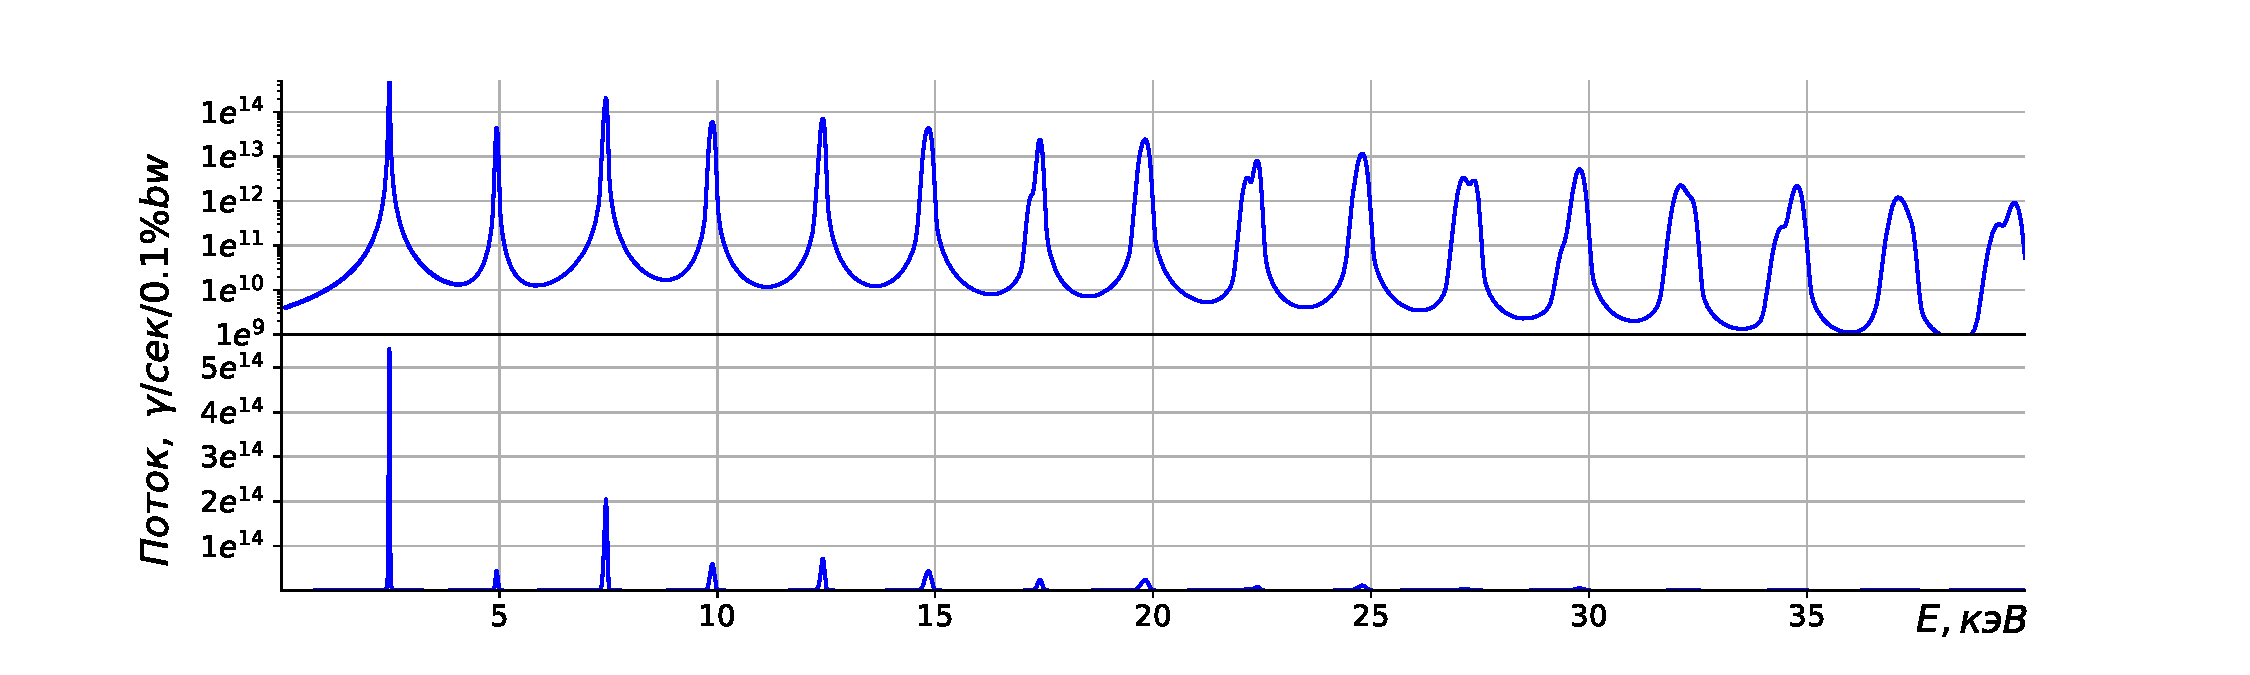
\includegraphics[width=\textwidth]{pic/log_spec_1-2.pdf}
	\caption{Спектр с ондулятора с $K = 1,54$ через апертуру $0,4 \; \textup{мм}$ в логарифмическом масштабе (сверху) и в линейном (снизу) посчитанный в SPECTRA}
	\label{fig:section_und_SRW}
\end{figure}

\subsection{Оптика станции 1-2}

\begin{figure}[h]
	\centering  
	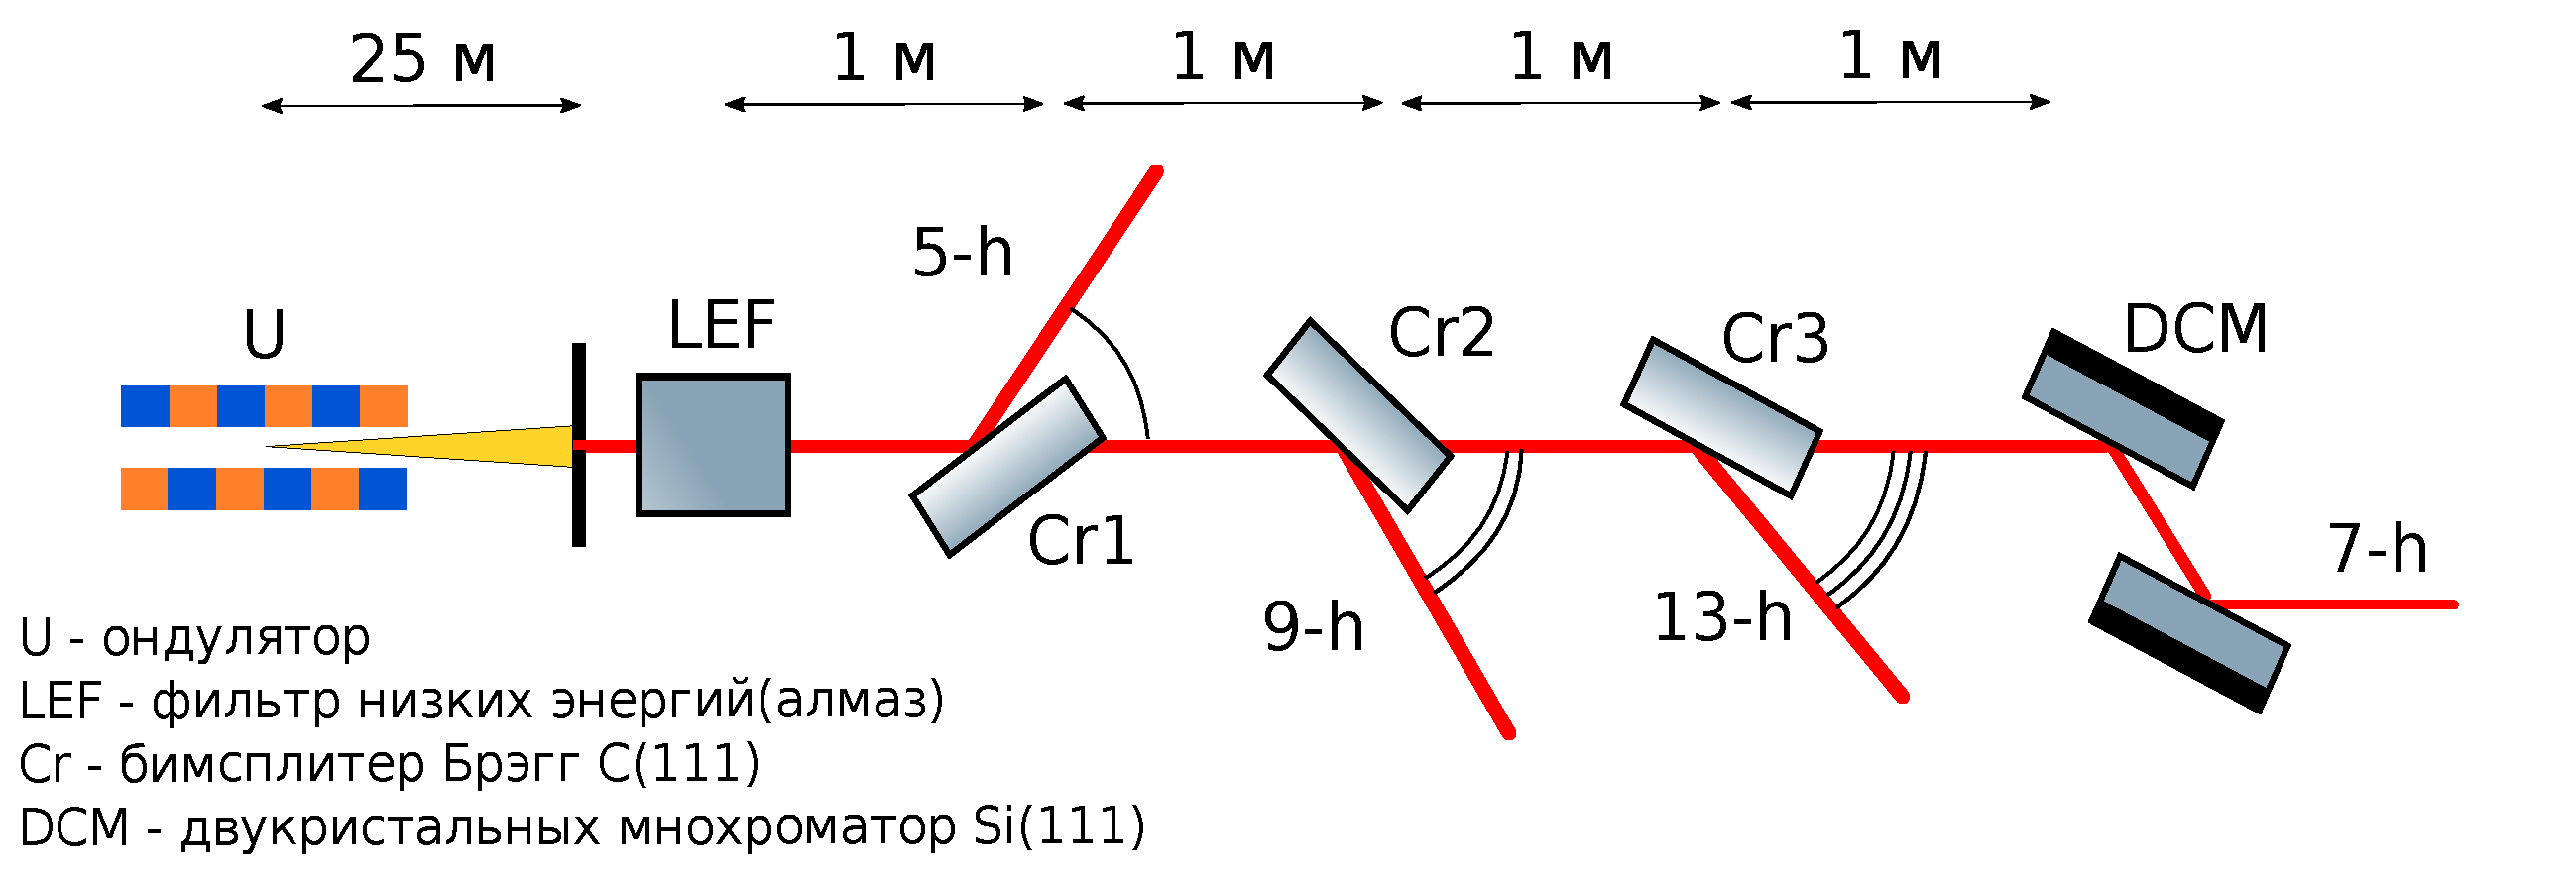
\includegraphics[width=\textwidth]{pic/OptScheme_1-2.pdf}
	\caption{Оптическая схема станции 1-2}
	\label{fig:OptScheme_1-2}  
\end{figure}


\section{Станция 1-4 --- <<XAFS-спектроскопия и магнитный дихроизм>>}
\subsection{Вставное устройство}
На вставное устройство станции 1-4 накладываются довольно жёсткие условия, так как на этой станции планируется реализовать две техники XAFS спектроскопии --- обычный EXAS и quick-EXAS. Последняя техника требует довольно широкого спектра до $1 - 1.2 \; \textup{кэВ}$, что не может быть реализованно с помощью обычного планарного ондулятора, ширина спектра которого, определяется количеством периодов и равна порядка: $\Delta \omega / \omega = 10^{-2}$. Для уширения спектра ондуляторного излучения используют так называемую технику тэперинга, изменение магнитного поля некоторым способом или длины периодов ондулятора вдоль траектории электронного пучка(ссылка).

На станции будет использоваться сверхпроводящий ондулятор с возможность производить сканирование по спектру. Магнитное поле может меняться в широких пределах, посредствам подстройки тока в обмотках сверхпроводящего устройства. Параметры такого ондулятор см. в таблице~\ref{table:und1-4}. 
\begin{table}[h!]
	\centering
	\begin{tabular}{c|c|c|c|c}
		\hline\hline
		\rule{0pt}{3ex}$\mathnormal{B(K), [T]}$   & $\mathnormal{L, [m]}$ & $\mathnormal{d, [mm]}$ & фаз.ошиб.                & Рабочие Гармоники       \\ \hline
		\rule{0pt}{3ex}$0.65 - 1.37(1.1 - 2.3)$   & $2.3$                 & $18$        		   & $ \leq 3^{\circ}$		  & $3 - 13$\\
		\hline\hline
	\end{tabular}
	\vspace{4pt} 
	\caption{Параметры ондулятора для станции 1-4}
	\label{table:und1-4}
\end{table}
Помимо этого, на  ондулятор накладывается условие того, что рабочие гармоники должны перекрываться, чтобы предоставить пользователям вести непрерывное сканирование по энергии в диапазоне от $4 \; \textup{кэВ}$ до $40 \; \textup{кэВ}$. На рис.~\ref{fig:F_A} представлен спектр с указанными выше $K$ ондулятора, показано эффективное перекрытие рабочих гармоник с большим запасом.
\begin{figure}[h!]
	\begin{minipage}{0.99\textwidth}
		\centering  
		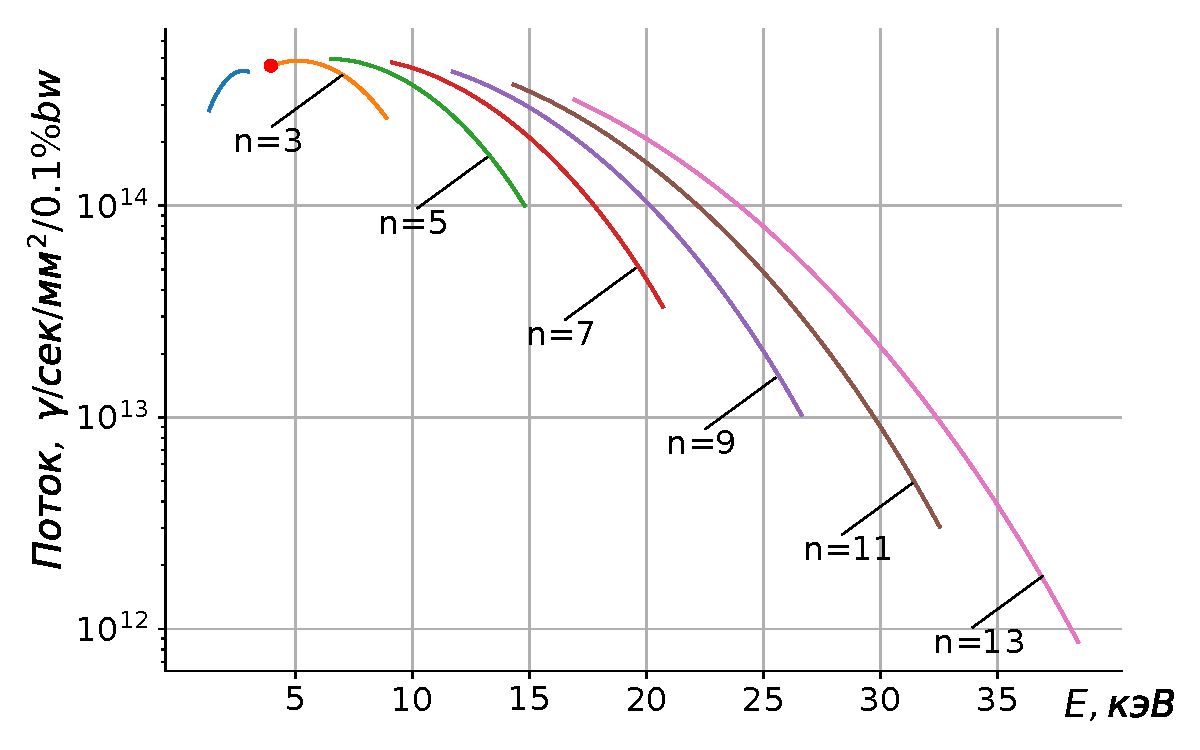
\includegraphics[width=\textwidth]{pic/F_A.pdf}
		\caption{Спектр ондулятора для 1-4 с параметром $K$ меняющемся в диапазоне от $1.1 - 2.3$}
		\label{fig:F_A}  
	\end{minipage}\hfill

	\begin{minipage}{0.99\textwidth}
		\centering
		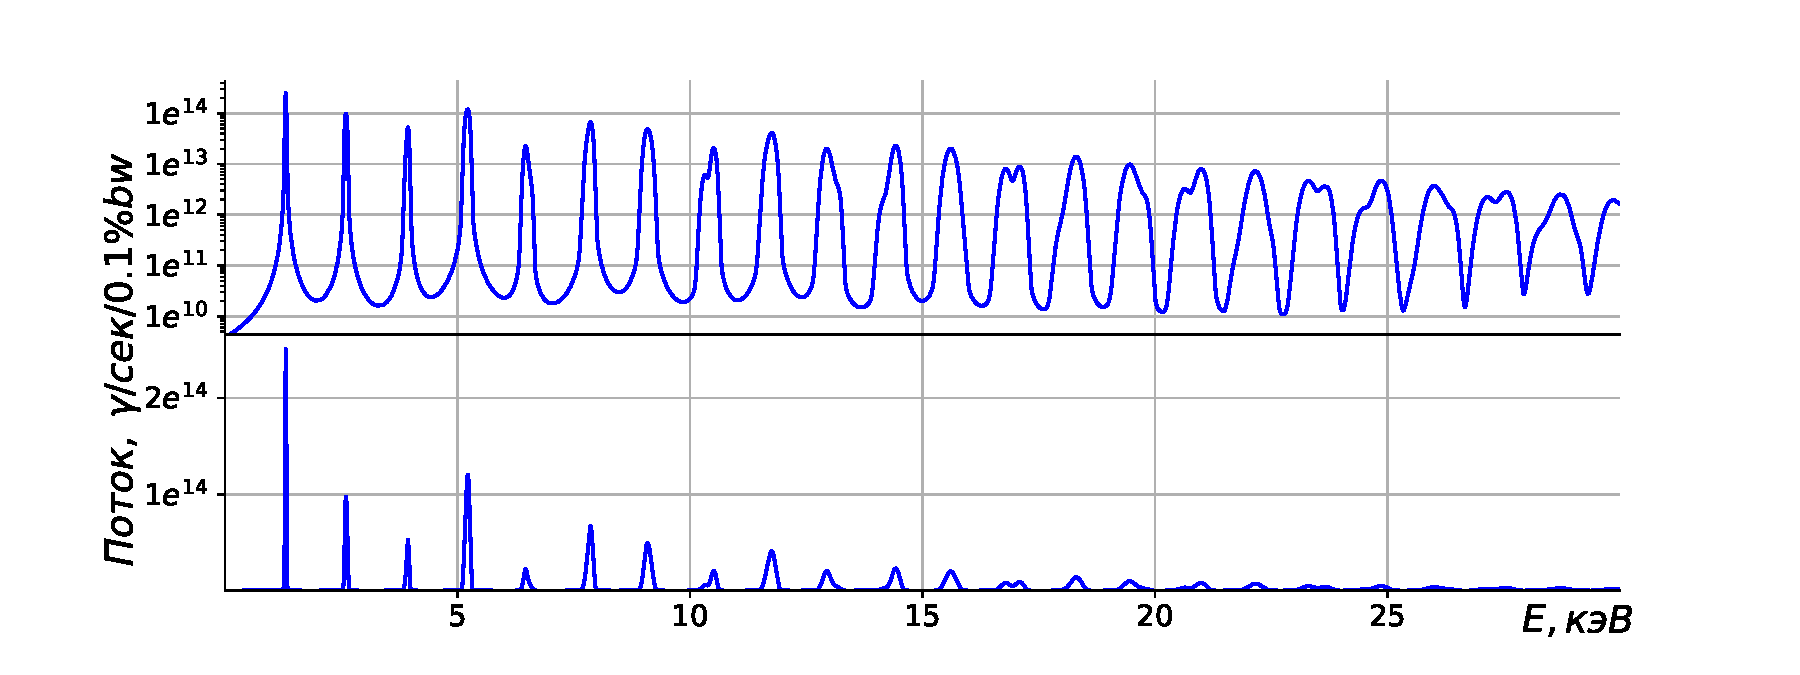
\includegraphics[width=\textwidth]{pic/log_spec_1-4.pdf}
		\caption{Спектр с ондулятора с $K = 2.23$ через апертуру $1 \; \textup{мм}$ в логарифмическом масштабе (сверху) и в линейном (снизу) посчитанный в SPECTRA}
		\label{fig:section_und_SRW}
	\end{minipage}    
\end{figure}


\subsection{Излучение клинообразного ондулятора}
В этой секции мы рассмотрим излучение планарного ондулятора специальной конструкции, который может доставить широкий спектр. Идея состоит в том, что разбить ондулятор на несколько секций с различным магнитным полем в каждой из них~\ref{fig:section_und_sheme}.
\begin{figure}[h]
	\centering  
	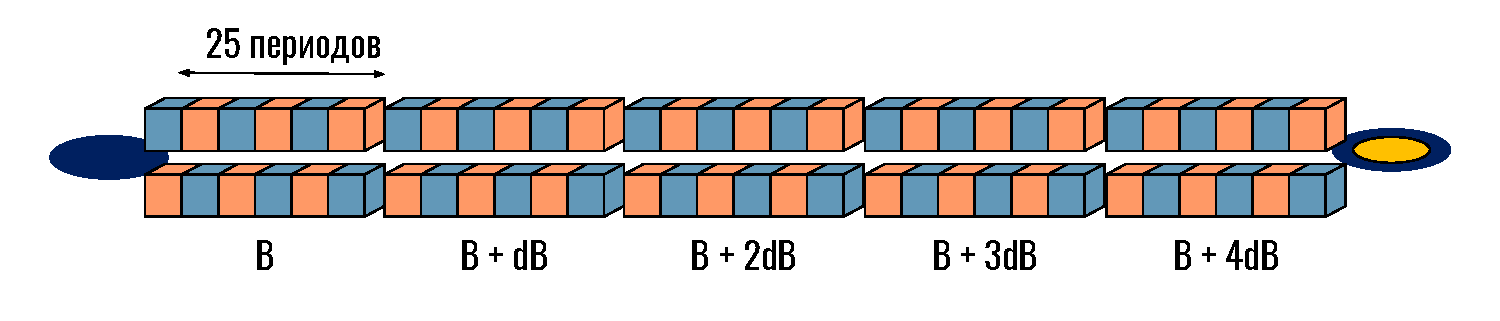
\includegraphics[width=\textwidth]{pic/und.pdf}
	\caption{Ондулятор состоящий из малых ондуляторных секций.}
	\label{fig:section_und_sheme}  
\end{figure}
Такая расстановка, в первом приближении, предполагалось должна дать набор резонансов, которые сольются в один сплошной спектр. Однако, более детальное рассмотрение показало, что в зависимости от фазы электрона между сегментами, могут проявляться интерференционные эффекты, которые в значительной степени будут изменять форму спектра. 

Выкладки можно начать с модифицированного интеграла~\ref{eq:field_dist_in_integral}, 
\begin{equation}
\begin{array}{lcl}
\vec{\widetilde{E}}_{\bot}(z_0,  \vec{r}_{\bot 0}, \omega) =
\cfrac{\omega eA_{JJ}}{2c^2z_0}\cfrac{K}{\gamma}
\displaystyle\int\limits_{-\lambda_w N/2}^{\lambda_w N/2} dz'
\exp[iCz'] 	\vec{e}_x,
\end{array}	
\end{equation} 
Здесь, для простоты изложения, излучение рассматривается на оси, т.е. $\theta = 0$ от уединённого электрона. В случае секционного ондулятора коэффициент ондуляторности меняется вдоль ондулятора, поэтому $K = K_0 + n\Delta K$, а также $C = C_0 + n\Delta C$, где $n$ --- это номер секции. Где $\Delta {C}$ введено следующим образом, помня $\omega_r = 2c\widetilde{\gamma}^2k_w$:
\begin{equation}
C =k_w\cfrac{\Delta \omega}{\omega_r} = \cfrac{\Delta \omega_r}{2c\gamma}\bigg(1 + \cfrac{(K_0 + n\Delta K)^2}{2}\bigg) \approx \cfrac{\Delta \omega_r}{2c\gamma}\bigg(1 + \cfrac{K^2_0}{2}(1 + \cfrac{n\Delta K}{K_0})\bigg) = C_0 + \Delta C
\end{equation} 
Секций, для определённости, мы возьмём пять, и для удобства нумерацию будем вести $-2, -1, ... , 2$. Поэтому интеграл можно переписать в виде:
\begin{equation}
\begin{array}{lcl}
\vec{\widetilde{E}}_{\bot}(z_0,  \vec{r}_{\bot 0}, \omega) =
\cfrac{\omega eA_{JJ}}{2c^2 \gamma z_0}
\displaystyle\sum\limits_{n =-2}^{2}(K_0 + n\Delta K)
\displaystyle\int\limits_{(2n + 1)L_s/2}^{(2n - 1)L_s/2} dz'
\exp[i(C_0 + n\Delta C)z']	\vec{e}_x,
\end{array}	
\end{equation} 
Взяв интеграл, получим:
\begin{equation}
\begin{array}{lcl}
\vec{\widetilde{E}}_{\bot}(z_0,  \vec{r}_{\bot 0}, \omega) =
\cfrac{\omega eA_{JJ} L}{2c^2 \gamma z_0}
\displaystyle\sum\limits_{n =-2}^{2}(K_0 + n\Delta K)
\sinc(\hat{C}/2)e^{in({C}_0 + n\Delta {C})L}	\vec{e}_x,
\end{array}	
\end{equation} 
Возведя в квадрат, получим интенсивность:
\begin{equation}
\begin{array}{lcl}
{\widetilde{I}} =
\bigg(\cfrac{\omega eA_{JJ} L}{2c^2 \gamma z_0}\bigg)^2\bigg[
\displaystyle\sum\limits_{n =-2}^{2}(K_0 + n\Delta K)^2\sinc^2(\hat{C_0} + n\Delta \hat{C}/2) \; + \\

\displaystyle\mathop{\sum\limits_{n, m =-2}^{2}}_{n \neq m}K^2_0\bigg(1 + n\cfrac{\Delta K}{K_0} + m\cfrac{\Delta K}{K_0}\bigg)
\sinc^2(\hat{C}/2)e^{i(n-m)\hat{C}_0 + (n^2 - m^2)\Delta \hat{C}}\bigg],
\end{array}	
\end{equation} 
Полученное выражение можно проинтерпретировать следующим образом: первая сумма есть сумма сдвинутых по соответствующим резонансам $\sinc^2$ функций, вторая сумма отображает интерференцию между различными секциями ондулятора. Данная комбинация приводит к колебаниями в спектре, как показано на рис.~\ref{fig:section_und_analitics} синими пунктирными линиями, чёрной линией отмечена сумма $\sinc^2$ функций без учёта интерференционных слагаемых.
\begin{figure}[h!]
	\centering  
	\begin{minipage}{0.49\textwidth}
		\centering
		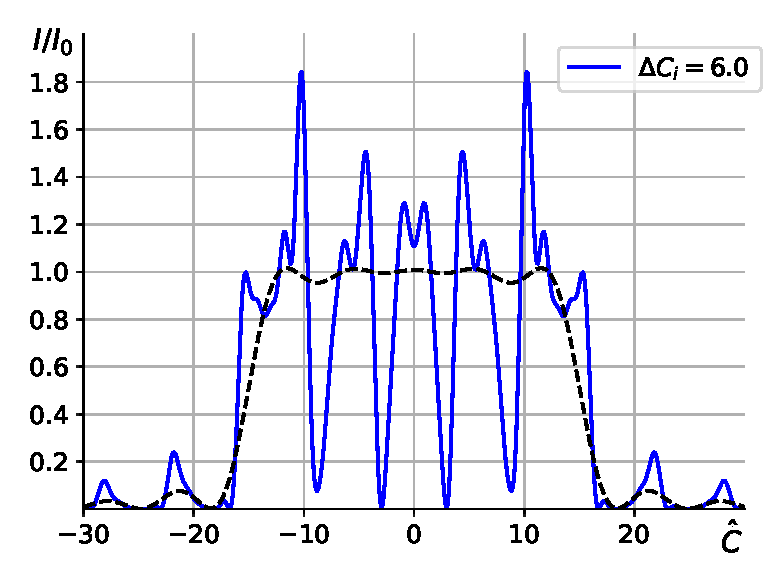
\includegraphics[width=\textwidth]{pic/spec_from_sec_und.pdf}
		\caption{Аналитический результат}
		\label{fig:section_und_analitics}
	\end{minipage}\hfill
	\begin{minipage}{0.49\textwidth}
		\centering
		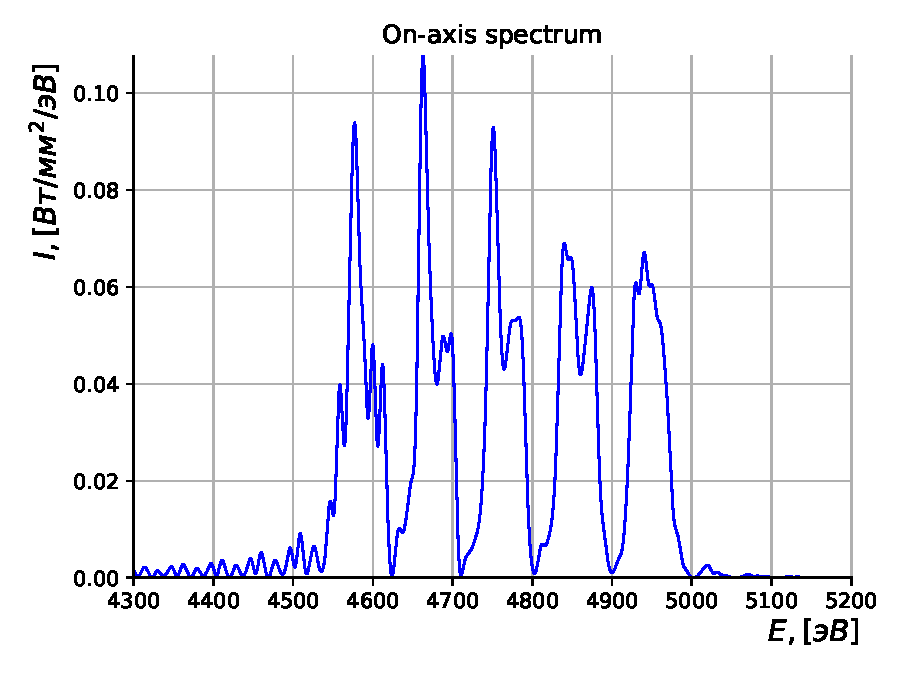
\includegraphics[width=\textwidth]{pic/sim_und_spec.pdf}
		\caption{Симуляция в коде SRW}
		\label{fig:section_und_SRW}
	\end{minipage}    
\end{figure}
На рис.~\ref{fig:section_und_SRW} показан характерный спектр секционного ондулятора посчитанного при помощи симуляционного кода SRW. Далее на рис.~\ref{fig:sim_und_spec_new_mm} представлен спектр с учётом эмиттанса и энергетического разброса в пучке, проинтегрированный по конечной апертуре --- $1 \; \textup{мм}$ на расстоянии $22 \; \textup{м}$.
\begin{figure}[h!]
	\centering  
	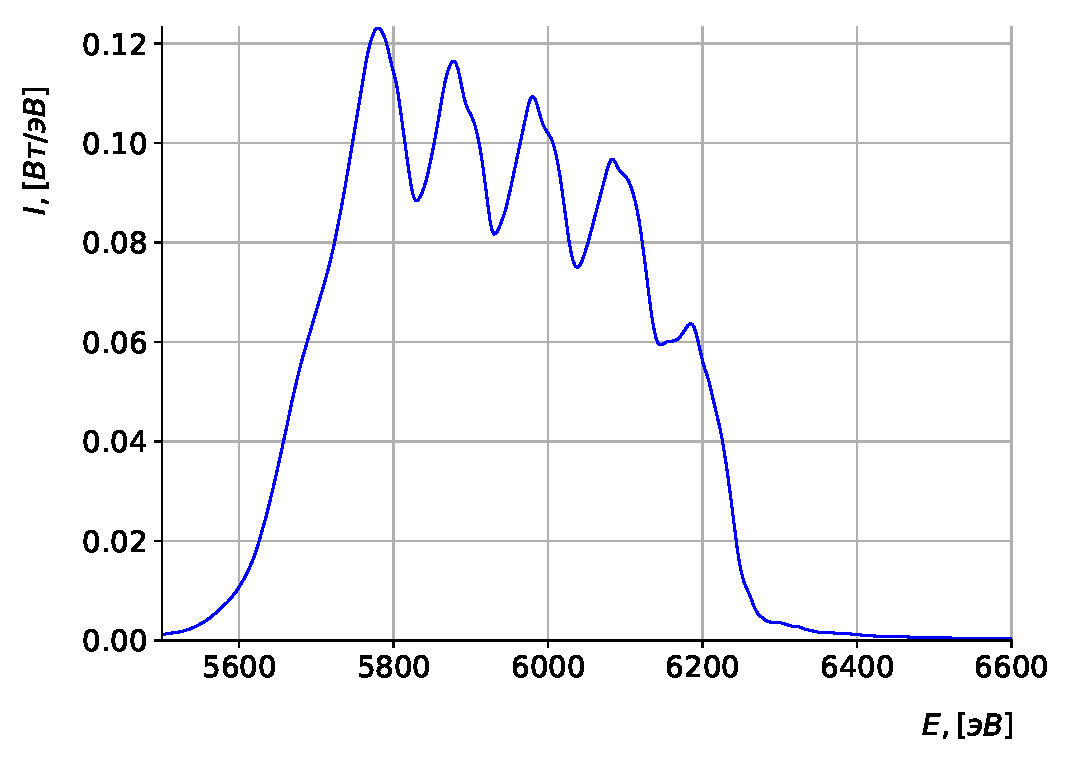
\includegraphics[width=\textwidth]{pic/sim_und_spec_new_mm.pdf}
	\caption{Спектр секционного ондулятора проинтегрированного по конечной апертуре --- $1 \; \textup{мм}$}
	\label{fig:sim_und_spec_new_mm}  
\end{figure}
\subsection{Оптика станции 1-4}

На рис.~\ref{fig:OptScheme_1-4} представленна оптическая схема станции реализации EXAS спектроскопии, которая состоит из двукристального монохроматора и далее системы зеркал Kirkpatrick-Baez для фокусировки излучения на образец. Для реализации quick-EXAS спектроскопии будет использоваться отдельный монохроматор, но т.к. на данный момент нет консенсуса по концепции ондулятора для этой техники, в данной работе оптическая схема для указанного метода рассматриваться не будет.

\begin{figure}[h]
	\begin{minipage}{0.99\textwidth}
	\centering  
	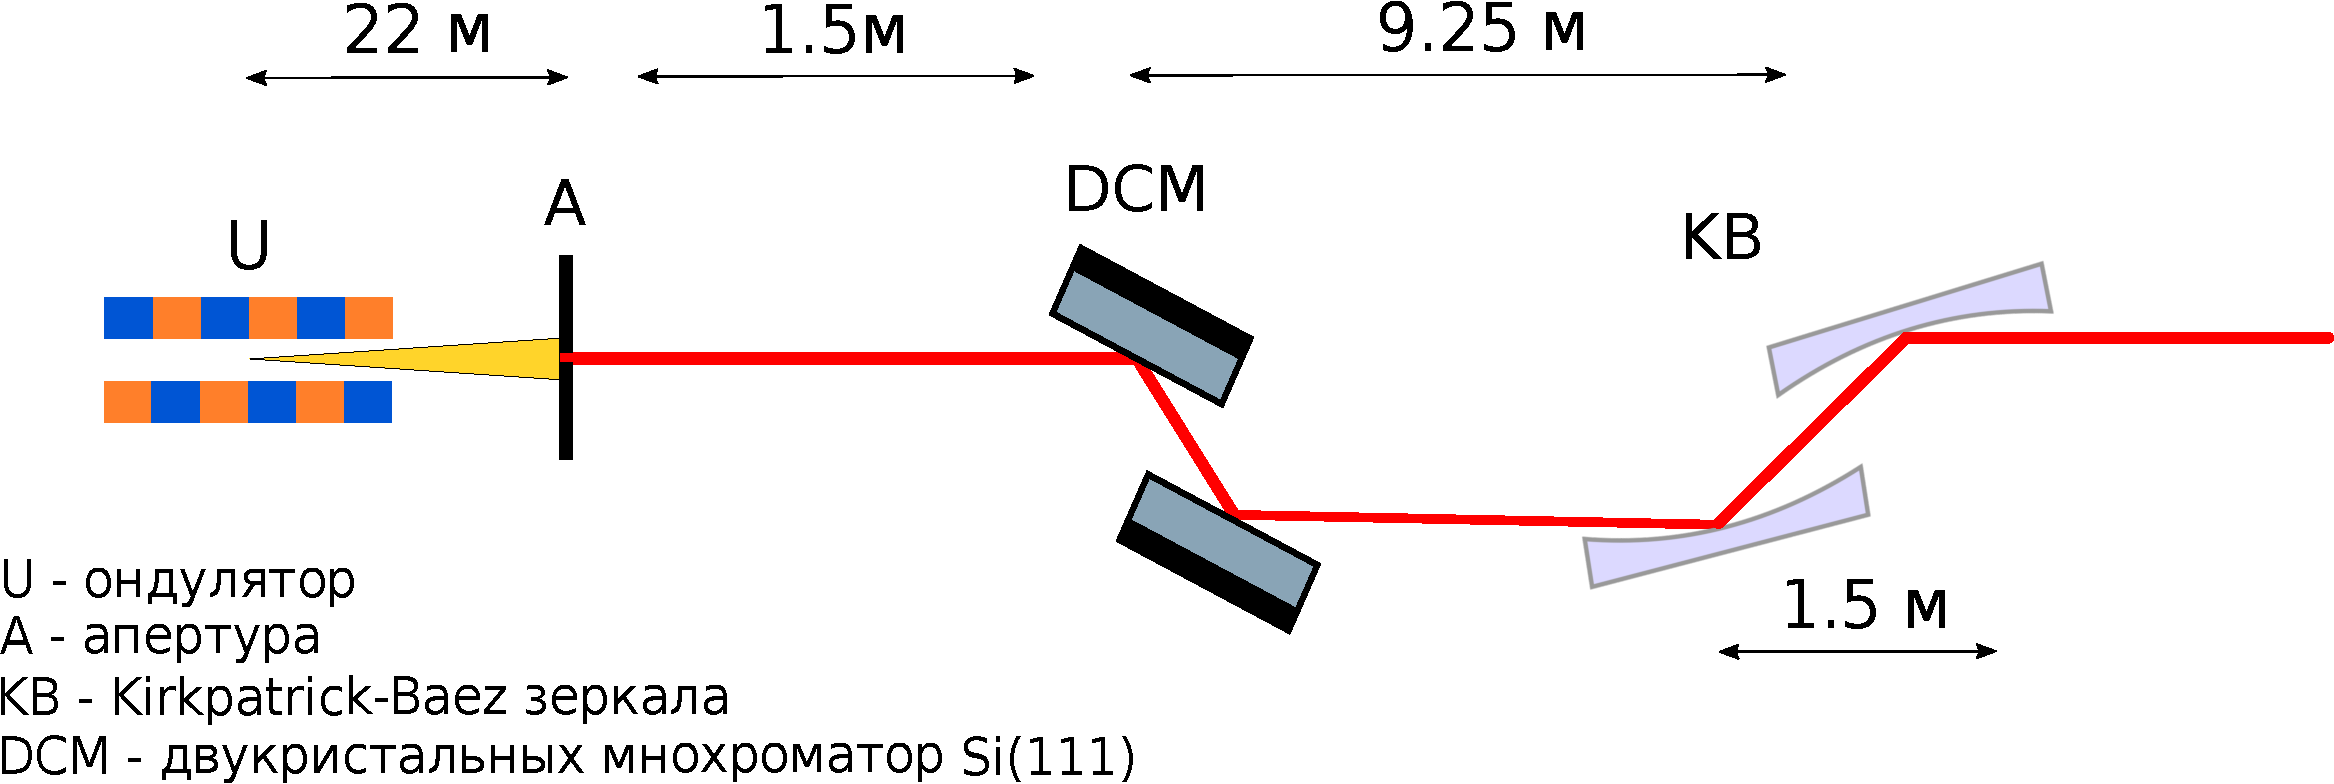
\includegraphics[width=\textwidth]{pic/OptScheme_1-4.pdf}
	\caption{Оптическая схема станции 1-4}
	\label{fig:OptScheme_1-4}  
	\end{minipage}\hfill

	\begin{minipage}{0.3\textwidth}
		\centering
		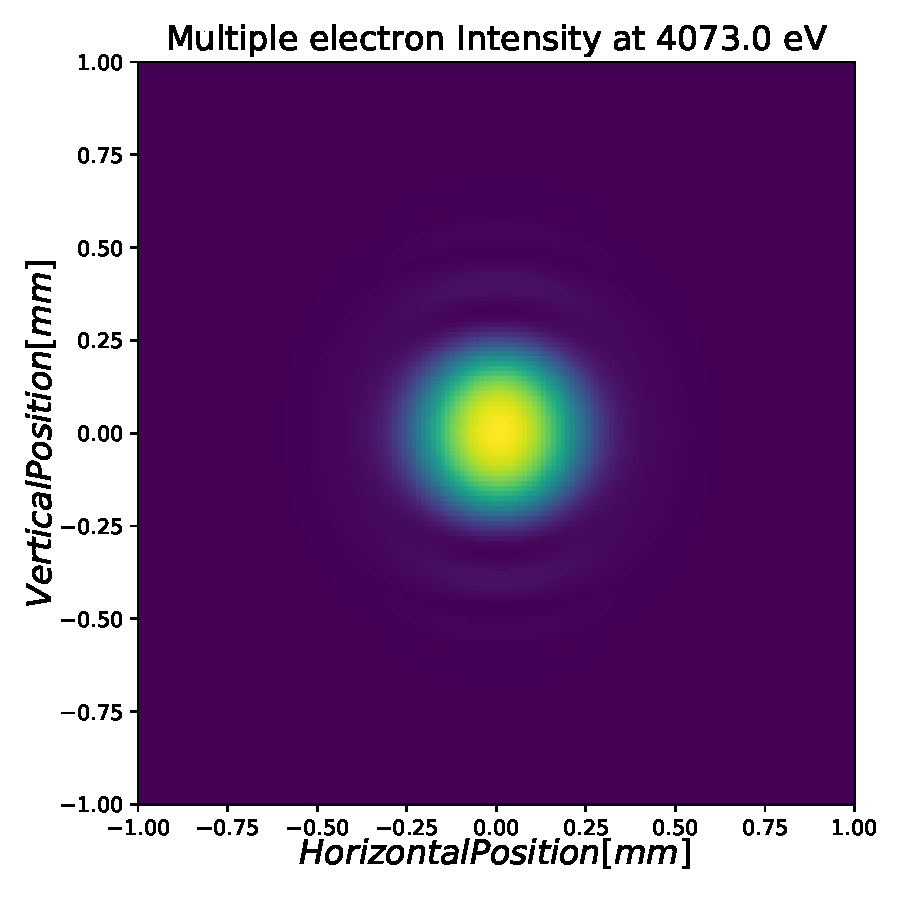
\includegraphics[width=\textwidth]{pic/3_harm_before_optics_2d.pdf}
		\caption{Сечение пучка до апертуры}
		\label{fig:3_harm_before_optics_2d}
	\end{minipage}
	\begin{minipage}{0.3\textwidth}
		\centering
		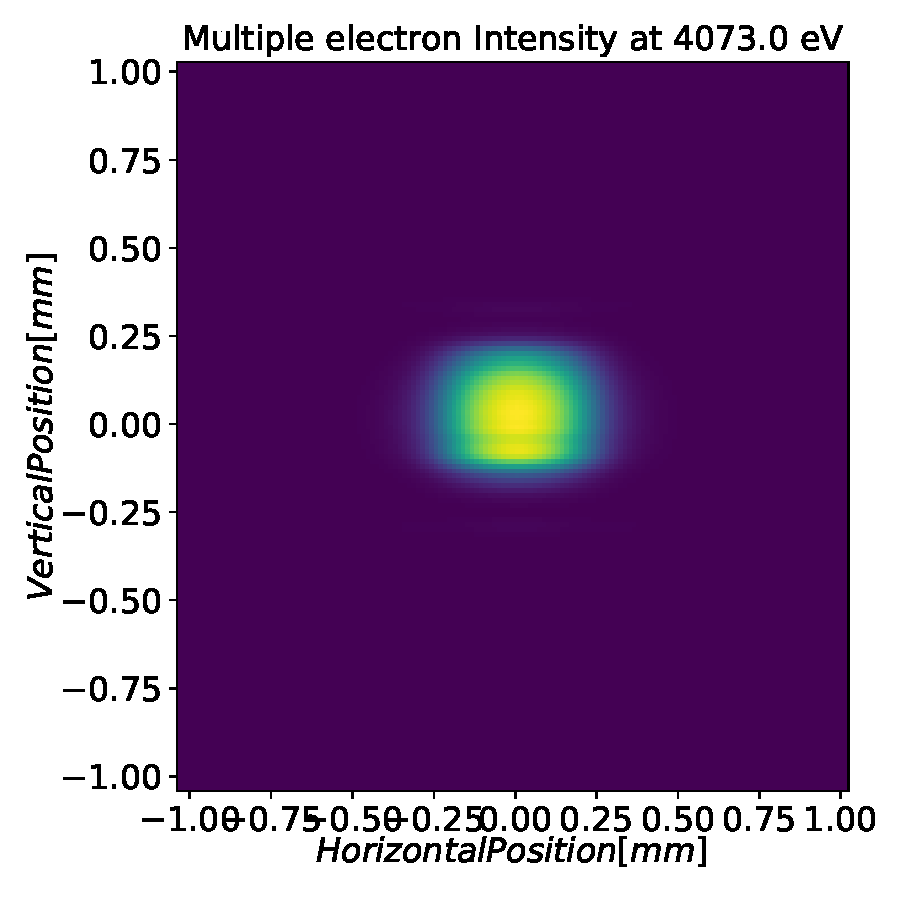
\includegraphics[width=\textwidth]{pic/3_harm_after_DCM_2d.pdf}
		\caption{Сечение пучка после DCM}
		\label{fig:3_harm_after_DCM_2d}
	\end{minipage} 
	\begin{minipage}{0.3\textwidth}
		\centering
		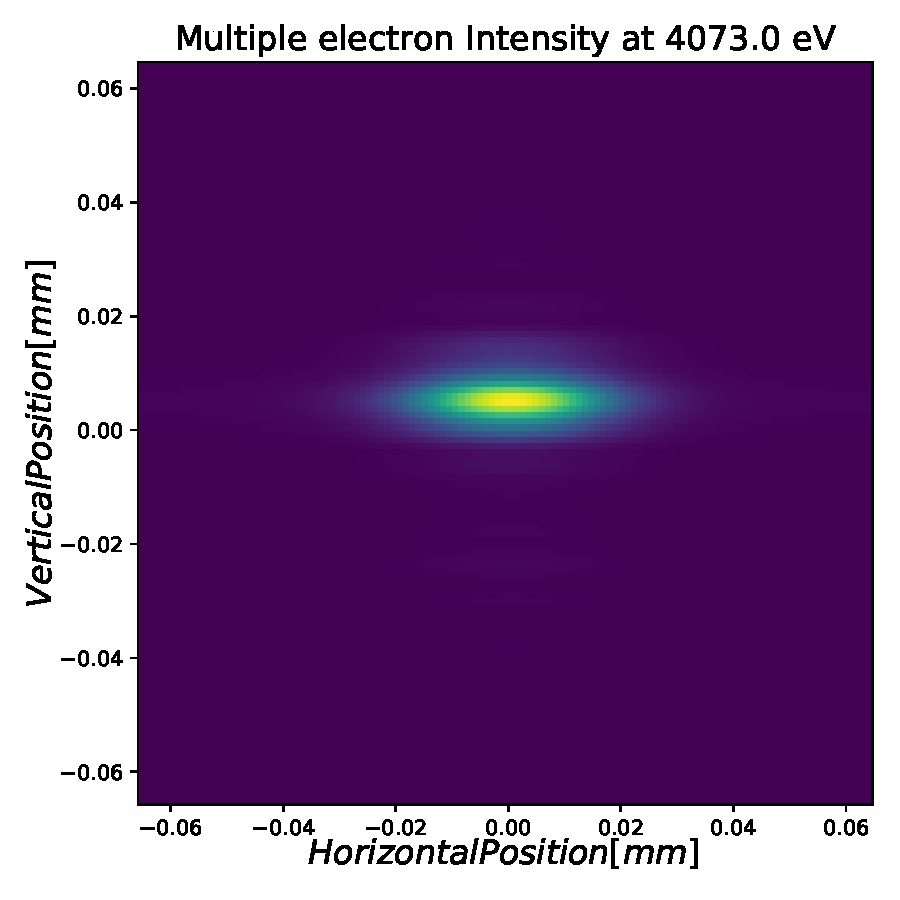
\includegraphics[width=\textwidth]{pic/3_harm_after_Sph_Mir_2d.pdf}
		\caption{Сечение пуска около фокуса зеркал}
		\label{fig:3_harm_after_Sph_Mir_2d}
	\end{minipage} 
\end{figure}
